
\chapter{漫谈SLAM}

摘录自 https://www.cnblogs.com/qcloud1001/p/7978238.html

https://cloud.tencent.com/developer/article/1005893

\section{漫谈 SLAM 技术(上)}
随着最近几年机器人、无人机、无人驾驶、VR/AR的火爆,SLAM技术也为大家熟知,被认为是这些领域的关键技术之一。本文对SLAM技术及其发展进行简要介绍,分析视觉SLAM系统的关键问题以及在实际应用中的难点,并对SLAM的未来进行展望。

\subsection{SLAM技术}

SLAM(Simultaneous Localization and Mapping),同步定位与地图构建,最早在机器人领域提出,它指的是:机器人从未知环境的未知地点出发,在运动过程中通过重复观测到的环境特征定位自身位置和姿态,再根据自身位置构建周围环境的增量式地图,从而达到同时定位和地图构建的目的。由于SLAM的重要学术价值和应用价值,一直以来都被认为是实现全自主移动机器人的关键技术。

如下图,通俗的来讲,SLAM回答两个问题:“我在哪儿?”“我周围是什么?”,就如同人到了一个陌生环境中一样,SLAM试图要解决的就是恢复出观察者自身和周围环境的相对空间关系,“我在哪儿”对应的就是定位问题,而“我周围是什么”对应的就是建图问题,给出周围环境的一个描述。回答了这两个问题,其实就完成了对自身和周边环境的空间认知。有了这个基础,就可以进行路径规划去达要去的目的地,在此过程中还需要及时的检测躲避遇到的障碍物,保证运行安全。

\begin{figure}[h]%%图
	\centering  %插入的图片居中表示
	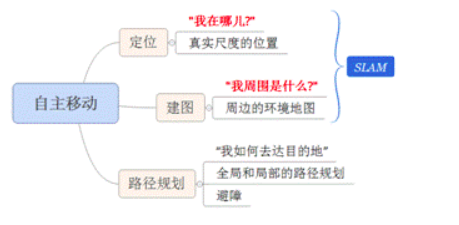
\includegraphics[width=0.7\linewidth]{image/Talk/1.png}  %插入的图,包括JPG,PNG,PDF,EPS等,放在源文件目录下
	\caption{SLAM概念}  %图片的名称
\end{figure}

\subsection{SLAM发展简介}
自从上世纪80年代SLAM概念的提出到现在,SLAM技术已经走过了30多年的历史。SLAM系统使用的传感器在不断拓展,从早期的声呐,到后来的2D/3D激光雷达,再到单目、双目、RGBD、ToF等各种相机,以及与惯性测量单元IMU等传感器的融合;SLAM的算法也从开始的基于滤波器的方法(EKF、PF等)向基于优化的方法转变,技术框架也从开始的单一线程向多线程演进。下面介绍这些过程中一些代表性的SLAM技术。

(1)激光雷达SLAM发展

基于激光雷达的SLAM(Lidar SLAM)采用2D或3D激光雷达(也叫单线或多线激光雷达),如下图所示。在室内机器人(如扫地机器人)上,一般使用2D激光雷达,在无人驾驶领域,一般使用3D激光雷达。


\begin{figure}[h]%%图
	\centering  %插入的图片居中表示
	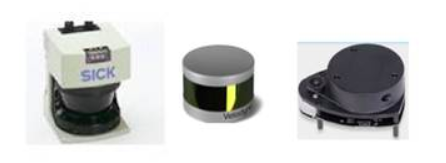
\includegraphics[width=0.7\linewidth]{image/Talk/2.png}  %插入的图,包括JPG,PNG,PDF,EPS等,放在源文件目录下

\end{figure}


激光雷达的优点是测量精确,能够比较精准的提供角度和距离信息,可以达到<1°的角度精度以及cm级别的测距精度,扫描范围广(通常能够覆盖平面内270°以上的范围),而且基于扫描振镜式的固态激光雷达(如Sick、Hokuyo等)可以达到较高的数据刷新率(20Hz以上),基本满足了实时操作的需要;缺点是价格比较昂贵(目前市面上比较便宜的机械旋转式单线激光雷达也得几千元),安装部署对结构有要求(要求扫描平面无遮挡)。

激光雷达SLAM建立的地图常常使用占据栅格地图(Ocupanccy Grid)表示,每个栅格以概率的形式表示被占据的概率,存储非常紧凑,特别适合于进行路径规划。

\begin{figure}[h]%%图
	\centering  %插入的图片居中表示
	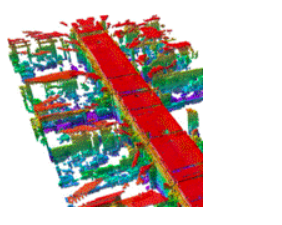
\includegraphics[width=0.7\linewidth]{image/Talk/3.png}  %插入的图,包括JPG,PNG,PDF,EPS等,放在源文件目录下
	\caption{激光雷达.}  %图片的名称
\end{figure}

现任Udacity创始人CEO、前Google副总裁、谷歌无人车领导者Sebastian Thrun大神(下图)在他2005年的经典著作《Probabilistic Robotics》一书中详细阐述了利用2D激光雷达基于概率方法进行地图构建和定位的理论基础,并阐述了基于RBPF粒子滤波器的FastSLAM方法,成为后来2D激光雷达建图的标准方法之一GMapping[1][2]的基础,该算法也被集成到机器人操作系统(Robot Operation System,ROS)中。
\begin{figure}[h]%%图
	\centering  %插入的图片居中表示
	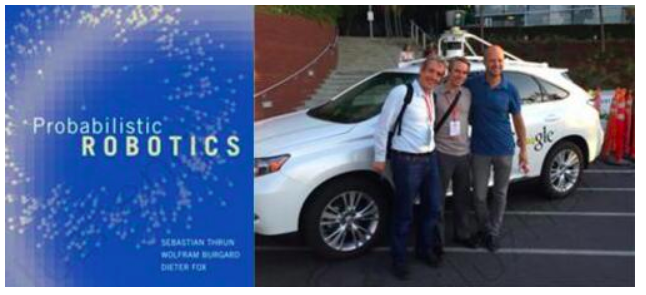
\includegraphics[width=0.7\linewidth]{image/Talk/4.png}  %插入的图,包括JPG,PNG,PDF,EPS等,放在源文件目录下

\end{figure}


2013年,文献[3]对ROS中的几种2D SLAM的算法HectorSLAM,KartoSLAM,CoreSLAM,LagoSLAM和GMapping做了比较评估,读者可前往细看。

2016年,Google开源其激光雷达SLAM算法库Cartographer[4],它改进了GMapping计算复杂,没有有效处理闭环的缺点,采用SubMap和Scan Match的思想构建地图,能够有效处理闭环,达到了较好的效果。

(2)视觉SLAM发展

相比于激光雷达,作为视觉SLAM传感器的相机更加便宜、轻便,而且随处可得(如人人都用的手机上都配有摄像头),另外图像能提供更加丰富的信息,特征区分度更高,缺点是图像信息的实时处理需要很高的计算能力。幸运的是随着计算硬件的能力提升,在小型PC和嵌入式设备,乃至移动设备上运行实时的视觉SLAM已经成为了可能。

视觉SLAM使用的传感器目前主要有单目相机、双目相机、RGBD相机三种,其中RGBD相机的深度信息有通过结构光原理计算的(如Kinect1代),也有通过投射红外pattern并利用双目红外相机来计算的(如Intel RealSense R200),也有通过TOF相机实现的(如Kinect2代),对用户来讲,这些类型的RGBD都可以输出RGB图像和Depth图像。

\begin{figure}[h]%%图
	\centering  %插入的图片居中表示
	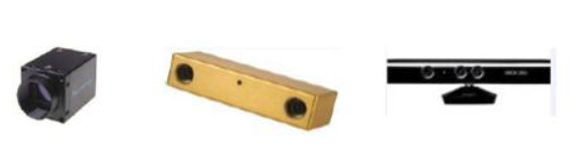
\includegraphics[width=0.7\linewidth]{image/Talk/5.png}  %插入的图,包括JPG,PNG,PDF,EPS等,放在源文件目录下

\end{figure}


现代流行的视觉SLAM系统大概可以分为前端和后端,如下图所示。前端完成数据关联,相当于VO(视觉里程计),研究帧与帧之间变换关系,主要完成实时的位姿跟踪,对输入的图像进行处理,计算姿态变化,同时也检测并处理闭环,当有IMU信息时,也可以参与融合计算(视觉惯性里程计VIO的做法);后端主要对前端的输出结果进行优化,利用滤波理论(EKF、PF等)或者优化理论进行树或图的优化,得到最优的位姿估计和地图。

\begin{figure}[h]%%图
	\centering  %插入的图片居中表示
	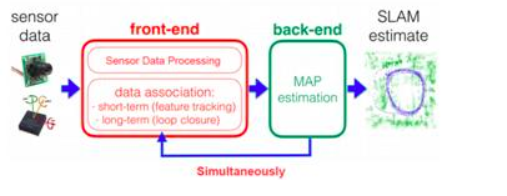
\includegraphics[width=0.7\linewidth]{image/Talk/6.png}  %插入的图,包括JPG,PNG,PDF,EPS等,放在源文件目录下

\end{figure}

采用滤波器的SLAM,如下图(a),估计n时刻的相机位姿Tn需要使用地图中所有路标的信息,而且每帧都需要更新这些路标的状态,随着新的路标的不断加入,状态矩阵的规模增长迅速,导致计算和求解耗时越来越严重,因此不适宜长时间大场景的操作;而采用优化算法的SLAM,如下图(b),通常结合关键帧使用,估计n时刻的相机位姿Tn可以使用整个地图的一个子集,不需要在每幅图像都更新地图数据,因此现代比较成功的实时SLAM系统大都采取优化的方法。
\begin{figure}[h]%%图
	\centering  %插入的图片居中表示
	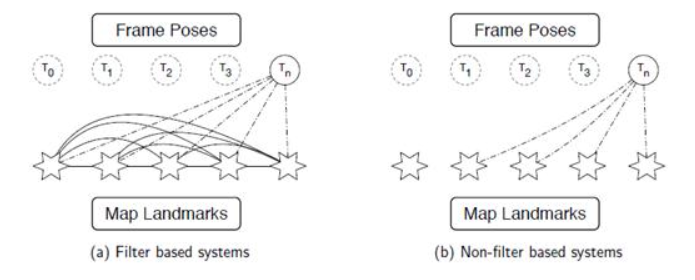
\includegraphics[width=0.7\linewidth]{image/Talk/7.png}  %插入的图,包括JPG,PNG,PDF,EPS等,放在源文件目录下

\end{figure}






下面介绍视觉SLAM发展历程中几个比较有代表性的SLAM系统进行介绍:

MonoSLAM[5]是2007年由Davison 等开发的第一个成功基于单目摄像头的纯视觉SLAM 系统。MonoSLAM使用了扩展卡尔曼滤波,它的状态由相机运动参数和所有三维点位置构成, 每一时刻的相机方位均带有一个概率偏差,每个三维点位置也带有一个概率偏差, 可以用一个三维椭球表示, 椭球中心为估计值, 椭球体积表明不确定程度(如下图所示),在此概率模型下, 场景点投影至图像的形状为一个投影概率椭圆。MonoSLAM 为每帧图像中抽取Shi-Tomasi角点[6], 在投影椭圆中主动搜索(active search)[7]特征点匹配。由于将三维点位置加入估计的状态变量中,则每一时刻的计算复杂度为O(n3) , 因此只能处理几百个点的小场景。
\begin{figure}[H]%%图
	\centering  %插入的图片居中表示
	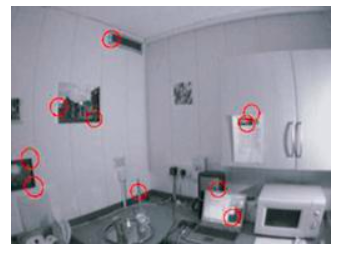
\includegraphics[width=0.7\linewidth]{image/Talk/8.png}  %插入的图,包括JPG,PNG,PDF,EPS等,放在源文件目录下

\end{figure}



同年,Davison在Oxford的师父Murray和Klein发表了实时SLAM系统PTAM(Parallel Tracking and Mapping)[8]并开源(如下图),它是首个基于关键帧BA的单目视觉SLAM 系统, 随后在2009 年移植到手机端上[9]。PTAM在架构上做出了创新的设计,它将姿态跟踪(Tracking)和建图(Mapping)两个线程分开并行进行,这在当时是一个创举,第一次让大家觉得对地图的优化可以整合到实时计算中,并且整个系统可以跑起来。这种设计为后来的实时SLAM(如ORB-SLAM)所效仿,成为了现代SLAM系统的标配。具体而言,姿态跟踪线程不修改地图,只是利用已知地图来快速跟踪;而建图线程专注于地图的建立、维护和更新。即使建立地图线程耗时稍长,姿态跟踪线程仍然有地图可以跟踪(如果设备还在已建成的地图范围内)。此外,PTAM还实现丢失重定位的策略,如果成功匹配点(Inliers)数不足(如因图像模糊、快速运动等)造成跟踪失败时,则开始重定位[10]——将当前帧与已有关键帧的缩略图进行比较,选择最相似的关键帧作为当前帧方位的预测。
\begin{figure}[H]%%图
	\centering  %插入的图片居中表示
	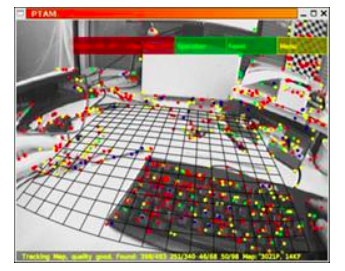
\includegraphics[width=0.7\linewidth]{image/Talk/9.png}  %插入的图,包括JPG,PNG,PDF,EPS等,放在源文件目录下

\end{figure}




2011年,Newcombe 等人提出了单目DTAM 系统[11], 其最显著的特点是能实时恢复场景三维模型(如下图)。基于三维模型,DTAM 既能允许AR应用中的虚拟物体与场景发生物理碰撞,又能保证在特征缺失、图像模糊等情况下稳定地直接跟踪。DTAM采用逆深度(Inverse Depth)[12]方式表达深度。如下图,DTAM将解空间离散为M×N×S 的三维网格,其中M× N为图像分辨率,S为逆深度分辨率,采用直接法构造能量函数进行优化求解。DTAM 对特征缺失、图像模糊有很好的鲁棒性,但由于DTAM 为每个像素都恢复稠密的深度图, 并且采用全局优化,因此计算量很大,即使采用GPU 加速, 模型的扩展效率仍然较低。
\begin{figure}[H]%%图
	\centering  %插入的图片居中表示
	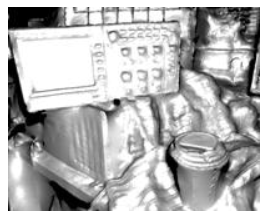
\includegraphics[width=0.7\linewidth]{image/Talk/10.png}  %插入的图,包括JPG,PNG,PDF,EPS等,放在源文件目录下

\end{figure}


2013年,TUM机器视觉组的Engel 等人提出了一套同样也是基于直接法的视觉里程计(visual odometry, VO)系统,该系统2014年扩展为视觉SLAM 系统LSD-SLAM[13],并开源了代码。与DTAM相比,LSD-SLAM 仅恢复半稠密深度图(如下图),且每个像素深度独立计算, 因此能达到很高的计算效率。LSD-SLAM 采用关键帧表达场景,每个关键帧K包含图像 Ik、逆深度图Dk和逆深度的方差Vk。系统假设每个像素x的逆深度值服从高斯分布N(Dk (x),Vk (x))。LSD-SLAM 的前台线程采用直接法计算当前帧t与关键帧k之间相对运动,后台线程对关键帧中每个半稠密抽取的像素点x(梯度显著区域), 在It中沿极线搜索Ik (x)的对应点, 得到新的逆深度观测值及其方差,然后采用EKF更新Dk和Vk 。LSD-SLAM采用位姿图优化来闭合回环和处理大尺度场景。2015年,Engel等人对LSD-SLAM进行了功能拓展,使其能够支持双目相机[14]和全景相机[15]。


\begin{figure}[H]%%图
	\centering  %插入的图片居中表示
	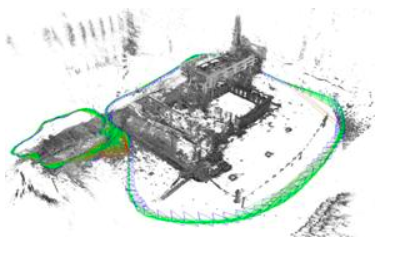
\includegraphics[width=0.7\linewidth]{image/Talk/11.png}  %插入的图,包括JPG,PNG,PDF,EPS等,放在源文件目录下

\end{figure}


2014年,苏黎世大学机器人感知组的Forster等人提出开源的SVO系统[16],该系统对稀疏的特征块使用直接法配准(Sparse Model-based Image Alignment),获取相机位姿,随后根据光度不变假设构造优化方程对预测的特征位置进行优化(Feature Alignment),最后对位姿和结构进行优化(Motion-only BA和Structure-only BA),而在深度估计方面,构造深度滤波器,采用一个特殊的贝叶斯网络[17]对深度进行更新。SVO的一个突出优点就是速度快,由于使用了稀疏的图像块,而且不需要进行特征描述子的计算,因此它可以达到很高的速度(作者在无人机的嵌入式ARM Cortex A9 4核1.6Ghz处理器平台上可以达到55fps的速度),但是SVO缺点也很明显,它没有考虑重定位和闭环,不算是一个完整意义上的SLAM系统,丢失后基本就挂了,而且它的Depth Filter收敛较慢,结果严重地依赖于准确的位姿估计;2016年,Forster对SVO进行改进,形成SVO2.0[18]版本,新的版本做出了很大的改进,增加了边缘的跟踪,并且考虑了IMU的运动先验信息,支持大视场角相机(如鱼眼相机和反射式全景相机)和多相机系统,该系统目前也开源了可执行版本[19];值得一提的是,Foster对VIO的理论也进行了详细的推导,相关的文献[20]成为后续SLAM融合IMU系统的理论指导,如后面的Visual Inertial ORBSLAM等系统。
\begin{figure}[H]%%图
	\centering  %插入的图片居中表示
	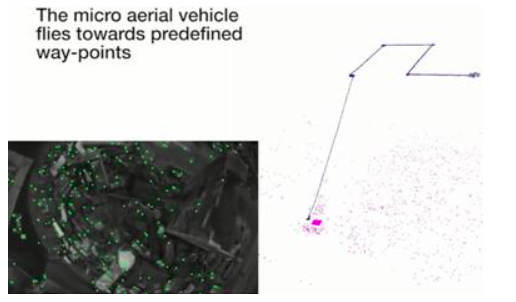
\includegraphics[width=0.7\linewidth]{image/Talk/12.png}  %插入的图,包括JPG,PNG,PDF,EPS等,放在源文件目录下

\end{figure}


2015年,Mur-Artal 等提出了开源的单目ORB-SLAM[21],并于2016年拓展为支持双目和RGBD传感器的ORB-SLAM2[22],它是目前支持传感器最全且性能最好的视觉SLAM系统之一,也是所有在KITTI数据集上提交结果的开源系统中排名最靠前的一个[23]。ORB-SLAM 延续了PTAM 的算法框架,增加了单独的回环检测线程,并对框架中的大部分组件都做了改进,归纳起来主要有以下几点:1)ORB-SLAM追踪、建图、重定位和回环检测各个环节都使用了统一的ORB 特征[24],使得建立的地图可以保存载入重复利用;2)得益于共视图(convisibility graph)的使用,将跟踪和建图操作集中在一个局部互见区域中,使其能够不依赖于整体地图的大小,能够实现大范围场景的实时操作;3)采用统一的BoW词袋模型进行重定位和闭环检测,并且建立索引来提高检测速度;4)改进了PTAM只能手工选择从平面场景初始化的不足,提出基于模型选择的新的自动鲁棒的系统初始化策略,允许从平面或非平面场景可靠地自动初始化。后来,Mur-Artal又将系统进行了拓展,形成了融合IMU信息的Visual Inertial ORB-SLAM[25],采用了Foster的论文[]提出的预积分的方法,对IMU的初始化过程和与视觉信息的联合优化做了阐述。
\begin{figure}[H]%%图
	\centering  %插入的图片居中表示
	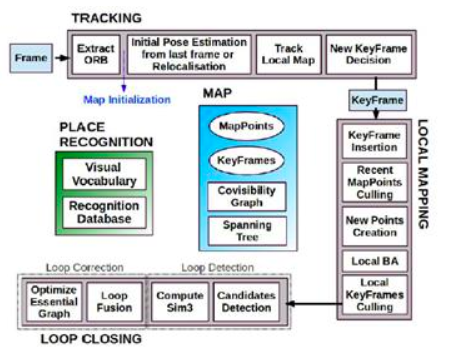
\includegraphics[width=0.7\linewidth]{image/Talk/13.png}  %插入的图,包括JPG,PNG,PDF,EPS等,放在源文件目录下

\end{figure}


2016年,LSD-SLAM的作者,TUM机器视觉组的Engel等人又提出了DSO系统[26]。该系统是一种新的基于直接法和稀疏法的视觉里程计,它将最小化光度误差模型和模型参数联合优化方法相结合。为了满足实时性,不对图像进行光滑处理,而是对整个图像均匀采样。DSO不进行关键点检测和特征描述子计算,而是在整个图像内采样具有强度梯度的像素点,包括白色墙壁上的边缘和强度平滑变化的像素点。而且,DSO提出了完整的光度标定方法,考虑了曝光时间,透镜晕影和非线性响应函数的影响。该系统在TUM monoVO、EuRoC MAV和ICL-NUIM三个数据集上进行了测试,达到了很高的跟踪精度和鲁棒性。
\begin{figure}[H]%%图
	\centering  %插入的图片居中表示
	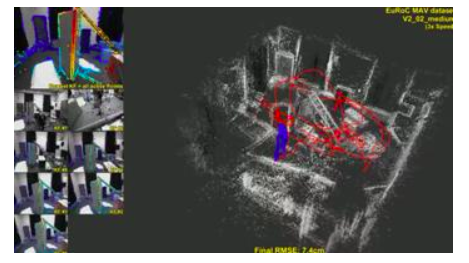
\includegraphics[width=0.7\linewidth]{image/Talk/14.png}  %插入的图,包括JPG,PNG,PDF,EPS等,放在源文件目录下

\end{figure}


2017年,香港科技大学的沈绍劼老师课题组提出了融合IMU和视觉信息的VINS系统[27],同时开源手机和Linux两个版本的代码,这是首个直接开源手机平台代码的视觉IMU融合SLAM系统。这个系统可以运行在iOS设备上,为手机端的增强现实应用提供精确的定位功能,同时该系统也在应用在了无人机控制上,并取得了较好的效果。VINS-Mobile使用滑动窗口优化方法,采用四元数姿态的方式完成视觉和IMU融合,并带有基于BoW的闭环检测模块,累计误差通过全局位姿图得到实时校正。
\begin{figure}[H]%%图
	\centering  %插入的图片居中表示
	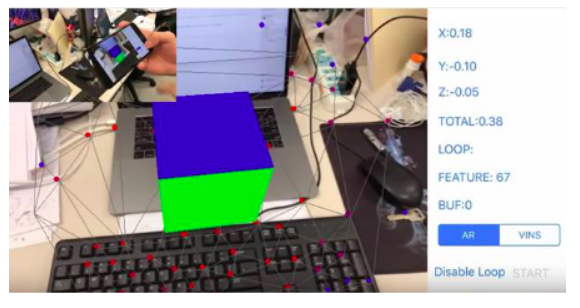
\includegraphics[width=0.7\linewidth]{image/Talk/15.png}  %插入的图,包括JPG,PNG,PDF,EPS等,放在源文件目录下

\end{figure}

\section{漫谈 SLAM 技术(下)}

\subsection{视觉SLAM系统关键问题}

结合上述介绍的SLAM系统,我们从以下几个方面分析视觉SLAM系统需要考虑的关键问题。

(1)图像信息使用

视觉SLAM方法根据使用图像信息的不同可分为直接法,间接法。

直接法,常见于稠密或半稠密的SLAM中,指的是采用图像上每个像素的信息(亮度值)来估计相机位姿;间接法,常用于稀疏的SLAM中,只使用显著的图像部位(即特征)用于位姿估计的计算。

直接法最基本的原理是亮度一致性约束,由于摄像机可以直接测量光的亮度,那么它的优化目标函数是光度误差(如下图),优化变量可以是两幅图像之间的位姿关系,也可以是特征Patch的位置。

\begin{figure}[H]%%图
	\centering  %插入的图片居中表示
	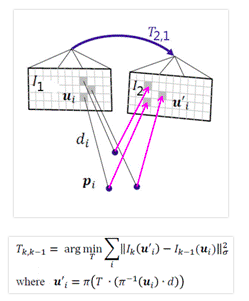
\includegraphics[width=0.7\linewidth]{image/Talk/16.png}  %插入的图,包括JPG,PNG,PDF,EPS等,放在源文件目录下

\end{figure}


根据直接法使用的像素的不同,可以分为稠密直接法和半稠密直接法。在上述介绍的SLAM系统中,DTAM为稠密直接法,它使用了所有的像素;LSD-SLAM和DSO为半稠密直接法,它使用了梯度明显的像素;SVO也为半稠密直接法,它使用了FAST特征点周围邻域的像素。直接方法较多的使用了图像上像素的信息,在纹理较差的部分比间接法更鲁棒。但当场景中的光照变化后,直接法容易失效,亮度一致性约束要求两幅图像之间的光度误差尽可能地小。

间接法使用图像中的特征(点或者线)进行匹配,然后根据匹配关系求解(如下图),它的优化目标函数是特征的重投影误差,优化的变量一般为相对位姿。间接法选取的特征一般要求比较显著,对视角和光照变化具有不变性,对模糊和噪声有一定的弹性,这需要在计算速度和特征质量上取得平衡。计算机视觉领域研究了很多不同的特征提取和特征描述,它们对旋转、尺度不变,和计算速度的性能都不一样。选择合适的特征依赖于平台的计算能力,视觉SLAM算法运行的环境,还有图像的帧率。可选的角点提取器如Harris角点(Harris and Stephens, 1988)、Shi-Tomasi角点(Shi and Tomasi, 1994),FAST角点(Mair et al, 2010)等,特征描述包括但不限于BRIEF,BRISK,SURF,SIFT,FREAK,ORB和像素级别局部区块特征等。
\begin{figure}[H]%%图
	\centering  %插入的图片居中表示
	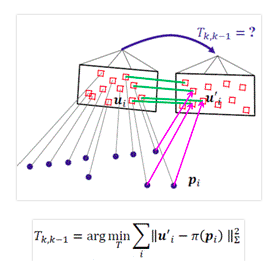
\includegraphics[width=0.7\linewidth]{image/Talk/17.png}  %插入的图,包括JPG,PNG,PDF,EPS等,放在源文件目录下

\end{figure}

使用间接法的SLAM系统一般都是稀疏的,因为它们只使用了图像的很少一部分像素的信息。在上述介绍的SLAM系统中,PTAM、ORBSLAM、VINS都属于间接法的SLAM系统。

(2)数据关联

数据关联就是在不同图像之间建立对应关系,也就是把在多个视角看到的同样的图像部分关联起来,这样才能为后续恢复三维结构做好基础。

特征对应主要有三类:2D-2D,3D-2D和3D-3D。

2D-2D的对应通常用于SLAM系统初始化的时机,这时没有地图,也没有两幅图像之间的相机变换,只能使用2D-2D的数据关联。为了减少计算时间,避免错误数据关联的可能性,可以用第一幅图像的特征2D位置定义一个搜索窗口在第2幅图像中进行搜索,并采用特征描述之间的相似度进行度量。对于像素描述子的局部区块,通常使用模板(patch)匹配中差值的平方和(SSD),或者为了增加对于光照变化的鲁棒性,使用零均值像素灰度差平方和 (ZMSSD),或者零均值归一化交叉相关(ZNCC);对于高层特征描述子,比如ORB,SIFT和SURF,可能会采用L1范数(向量中各个元素绝对值之和,就是绝对值相加,又称曼哈顿距离),L2范数(就是欧几里德距离)或汉明距离,为了加速匹配的搜索过程,可以采用KD树或词袋(BoW)。

3D-2D的特征对应常用于SLAM系统的运行阶段,前一相机位姿估计和场景3D结构已知,需要估计2D特征和这些3D路标在图像中投影的对应关系,有了这个对应关系,就可以通过PnP的方法来求解当前图像和上一帧之间的相对位姿,通常计算PnP时为了排除外点的干扰会结合RANSAC的方法进行。

3D-3D的数据对应主要用来估计和校正回环的累积误差,计算能使回环对齐的相似变换。在RGBD或双目系统中,还可以利用两帧之间的3D结构信息进行三维ICP配准来计算相对位姿,实现三维结构的对齐。

(3)初始化

单目的SLAM系统需要进行初始化,因为单帧图像数据并不能获取深度信息,也不能生成初始的地图。而RGBD和双目的SLAM系统由于单帧图像数据即可获取深度信息,所以不需要进行初始化操作。单目SLAM的初始化,只知道两幅图像之间的关联数据,初始相机位姿和场景结构都是未知的。

早期的MonoSLAM,系统初始化利用一个已知尺寸的平面矩形实现,将相机摆放在该矩形前已知距离的地方,利用平面矩形的四个角点计算初始位姿。

后来的SLAM系统,包括PTAM、SVO、ORBSLAM,都采用如下的流程进行初始化。
\begin{figure}[H]%%图
	\centering  %插入的图片居中表示
	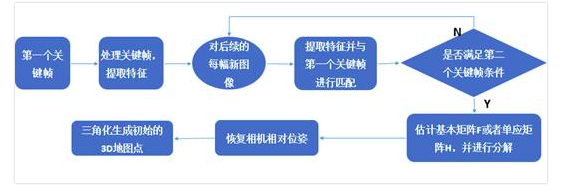
\includegraphics[width=0.7\linewidth]{image/Talk/18.png}  %插入的图,包括JPG,PNG,PDF,EPS等,放在源文件目录下

\end{figure}


PTAM使用单应矩阵初始化,此时场景应该由2D平面组成。PTAM要求用户手工选择前两个关键帧,而且用户在第一个和第二个关键帧之间,需要与场景平行地执行一个缓慢平滑且相对明显的平移运动。PTAM从第1个关键帧提取FAST特征点,在后来的每一帧图像中,采用2D-2D数据关联方法追踪,直到用户插入第2个关键帧。 特征匹配采用ZMSSD,由于没有考虑图像形变,匹配过程对运动模糊和由于相机旋转比较敏感,因此在初始化过程中对用户的运动状态要求比较严格。为了使匹配错误最小化,特征需要在两帧之间对称搜索,如果两个方向的匹配不一致,特征就会被丢弃。第2个关键帧成功加入之后,则采用MLESAC28的方法来计算两个关键帧之间的单应矩阵H,随后利用文献29的方法对H进行分解来恢复相机相对位姿。PTAM初始化非常脆弱,需要技巧去运行,尤其是对于没有经验的用户。另外,当初始化场景不是二维平面,或用户运动状态不恰当的时候,系统退化,容易崩溃。

SVO也使用单应矩阵进行初始化,但SVO不需要用户输入,系统启动时获取第一个关键帧并提取FAST特征,然后用图像间的KLT算法跟踪特征,为了避免用户二次输入,SVO实时检测第一个关键帧和当前图像间的特征点平移量的中值,当这个值达到一定的阈值,算法认为已经获得了足够的视差,开始估计单应矩阵,然后分解单应矩阵并校验相机位姿,得到正确的位姿估计,并三角化对应的内点形成地图点。在第二个图像作为关键帧加入地图管理线程之前,利用捆集调整优化这两个图像帧以及其关联的地图点。与PTAM一样,SVO的初始化同样要求平面场景。

LSD-SLAM的初始化不需要使用两视图几何,它从第1个视角随机初始化场景的深度,然后通过随后的图像不断对场景深度进行修正。图像中梯度明显的像素点的深度被初始化为随机的分布,并赋值为较大的方差后放入系统。第一个初始化的关键帧和后面的图像配准后,跟踪直接开始。图像不断输入,初始特征点的深度测量用滤波方法优化,直到收敛。这种方法不存在两视图几何的退化问题;但在深度收敛之前需要处理大量图像,需要一个中间跟踪过程,生成的地图也不可靠。

在ORB-SLAM中,为了解决上述问题,作者建议并行计算基本矩阵和单应矩阵(用RANSAC方法),并评估两种方法的对称传输误差来选择合适的模型。完成之后,就会进行适当的分解,恢复出相机的位姿,并三角化生成初始地图点,最后通过捆集调整优化地图。如果选择的模型导致跟踪质量差,或者图像上的特征匹配较少,初始化就会迅速被系统丢弃,重新进行初始化,这保证了初始化的可靠性。

(4)位姿估计

因为数据关联计算量巨大,对于每个新图像的位姿,如果能够有个位姿先验,那么对于缩小数据关联的范围就会非常有益。所以,建立这么一个先验是大部分SLAM系统位姿估计的第一个任务。PTAM,ORB SLAM,都在平滑的相机运动状态下采用恒定速度运动模型作为当前图像位姿的先验。但是,在相机运动方向上突然改变时,这样的模型就容易失效。LSD-SLAM和SVO都假设在随后的图像上(这种情况下都是用高帧率相机)相机位姿没有明显改变,因此它们给当前图像位姿和前一个跟踪到的图像分配相同的先验信息。

下图是位姿估计的流程,前一幅图像的位姿用于指导数据关联流程,它可以帮助从当前地图中提取可见的子图,从而减少盲目投影整个地图的计算开销;另外,它还可以为当前图像位姿提供先验,这样特征匹配只在很小的区域内进行搜索,而不是搜索整个图像;最后,它还可以作为优化相机位姿的迭代初值。
\begin{figure}[H]%%图
	\centering  %插入的图片居中表示
	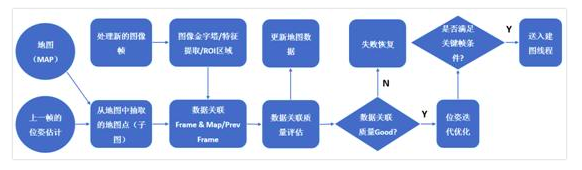
\includegraphics[width=0.7\linewidth]{image/Talk/19.png}  %插入的图,包括JPG,PNG,PDF,EPS等,放在源文件目录下

\end{figure}

下图演示了间接法的相机位姿是如何估计的,Cm是用运动模型估计的新图像位姿,C2是真实的相机位姿。利用Cm,将上一帧可见的地图点重投影到新图像上,在投影点周围一个搜索窗口Sw内进行数据关联,系统使用欧式变换参数(SE3变换)最小化重投影误差d。为了获得对外点(错误匹配的特征)的鲁棒性,目标函数最小化会利用核函数处理掉重投影误差比较大的特征。
\begin{figure}[H]%%图
	\centering  %插入的图片居中表示
	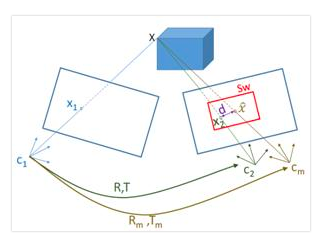
\includegraphics[width=0.7\linewidth]{image/Talk/20.png}  %插入的图,包括JPG,PNG,PDF,EPS等,放在源文件目录下

\end{figure}


(5)地图构建

不同的SLAM系统采用的地图表示形式不同,对于直接法的SLAM系统,由于恢复所有像素或者像素块的三维信息,它们生成地图为稠密或者半稠密的地图;而对于间接法的SLAM系统,它们仅恢复特征点的三维信息,生成的地图为稀疏的地图。无论是稠密、半稠密还是稀疏的地图,都可以看做三维的点云,虽然点云可以存储地图点的位置、特征和法线等,但是它们却不能反映相机位姿之间的关联,所以在SLAM系统中引入了位姿图(Pose Graph),如LSD-SLAM、ORB-SLAM。为了构建位姿图,SLAM系统会从图像帧中挑选一些帧作为关键帧,这些关键帧即为真实场景在不同位姿处的快照。关键帧包含了位姿信息和与地图点云的观测关系,这些关键帧构成了位姿图顶点,它们之间的连接构成了位姿图的边,两个关键帧之间共视的地图点的个数就是这条边的权值。

下图是地图构建的一般流程。可以看到地图构建需要处理两个方面的工作:新的地图元素的加入和已有地图数据的维护。
\begin{figure}[H]%%图
	\centering  %插入的图片居中表示
	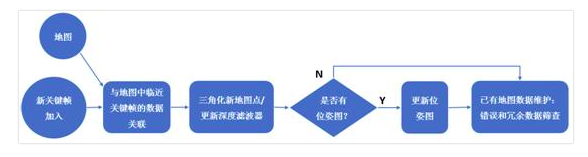
\includegraphics[width=0.7\linewidth]{image/Talk/21.png}  %插入的图,包括JPG,PNG,PDF,EPS等,放在源文件目录下

\end{figure}
新地图元素的加入主要是三维地图点和关键帧。现代的SLAM系统一般都会选取适当的关键帧,以达到场景的精简表示(如PTAM、SVO、LSD-SLAM通过明显的位姿变化原则添加新关键帧,ORB-SLAM通过明显的场景视图变化原则添加新关键帧);在新地图点生成方面,PTAM和ORB-SLAM通过优化关键帧位姿,根据匹配点三角化生成新的地图点,而SVO和LSD-SLAM通过图像帧与关键帧的匹配不断更新深度滤波器,最后利用收敛的特征点的深度来描述新地图点。

已有地图数据的维护主要采用优化的方法对关键帧和地图点位姿进行优化,减少累积误差,并对冗余或错误的关键帧和地图点进行筛除,维护地图数据的有效性和正确性。由于地图数据维护多采用局部BA和全局BA的方法,计算较为耗时,PTAM、LSD-SLAM和ORB-SLAM均单独开辟线程进行处理。

(6)重定位

重定位解决SLAM系统在遭遇突然的剧烈运动或者无特征区域等情况时,跟踪丢失后重新找回的问题。如果不能有效的重定位,SLAM系统前面建立的地图就不能再利用,系统就会失败。

PTAM在检测到跟踪失败后,会将后续每一帧的缩略图SBI(Small Blurry Image)与所有关键帧的SBI进行比较,如果与其灰度的差异小于一定的阈值,那么通过ESM方法估计其相对旋转,然后将地图点投影到当前帧寻找匹配,如果匹配足够,则计算精确位姿,重定位成功。这种方法需要丢失时的位姿与已有关键帧的位姿比较相近才可以成功,在有大的平移时会失败。

SVO简单将图像帧与丢失前最后一次有效位姿附近最近的关键帧进行匹配,如果匹配成功则重定位成功。这种重定位策略对于光照变化和大的平移都很敏感,很容易失败。

LSD-SLAM随机从位姿图中选择一个具有两个以上相邻关键帧的关键帧,并试图将当前帧与它进行匹配,如果外点/内点比率较大,那么丢弃该关键帧,重新随机选择;否则接着测试所有与它相邻的关键帧,如果相邻的关键帧中内点/外点比率较大的关键帧数多于外点/内点比率较大的关键帧数,或者存在多于五个的内点/外点比率较大的关键帧,那么选择内点/外点比率最大的关键帧进行跟踪,重定位成功。

ORB-SLAM的重定位会调用它的位置识别模块,该模块基于BoW进行,它计算当前图像的BoW向量,与地图中所有关键帧的BoW向量比较,找出所有匹配得分高于75%最好低分的关键帧作为候选。对这些候选进行匹配和RANSAC PnP计算,如果内点满足阈值条件,就认为重定位成功。

(7)回环检测

回环检测对于消除SLAM系统长时间运行的漂移有非常重要的作用,如果能够识别到过的地方,那么回环的两端就可以对齐,全局的尺度一致性就能够保证。

LSD-SLAM的做法是每当加入一个新关键帧时,通过FABMAP (Glover et al, 2012)中的Appearance Bbased model搜索与空间最近的10个关键帧的匹配,一旦检测到闭环,则对位姿图进行优化,计算相似变换对齐回环两端,并将回环误差分散到到各个关键帧中。

ORB-SLAM回环检测使用重定位时同样的基于BoW的地点识别模块,它可以为新加入的关键帧从已有关键帧数据库中高效快速的提取回环候选。为了确信回环和排除干扰,它引入连续一致性约束。确信回环之后,同样计算一个相似变换对齐回环两端。然后对关键帧和地图点进行调整,融合重复的地图点,并且执行一个基于位姿图的全局优化。

4. SLAM的实现难点
在《SLAM for Dummy》中,有一句话说的好:“SLAM并不是一种算法,而是一个概念”。(SLAM is more like a concept than a single algorithm.)

SLAM是多个学科多个算法的不同策略组合,它融合了图像处理,几何学,图理论,优化和概率估计等学科的知识,需要扎实的矩阵、微积分、数值计算知识,SLAM跟使用的传感器和硬件平台也有关系,研究者需要具备一定的硬件知识,了解所使用的传感器的硬件特性。所以,根据不同的应用场景,SLAM研究者和工程师必须处理从传感器模型构建到系统集成的各种实践问题。

从上面章节的分析可以看出,SLAM的各个环节用到的技术是偏传统的。与当前大热的深度学习“黑箱模型”不同,SLAM的各个环节基本都是白箱,能够解释得非常清楚。但SLAM却并不是上述各种算法的简单叠加,而是一个系统工程,里面有很多TradeOff。

比如SLAM需要平衡实时性和准确性,SLAM一般是多线程并发执行,资源的分配、读写的协调、地图数据的管理、优化和准确性、关键参数和变量的不确定性以及高速高精度度的姿态跟踪等,都是需要解决的问题。

SLAM还需要考虑硬件的适配,SLAM的数据来源于传感器,有时是多个传感器融合,传感器的质量对SLAM的效果影响很大。例如,如果SLAM使用的相机图像噪点非常多,那么就会对姿态跟踪产生不好的影响,因为特征点提取会很不一致;再比如在VIO系统中,如果相机和IMU的时间戳不一致(至少毫秒级),也会影响算法精度甚至算法失败。多个传感器的分别校准和互相校准,乃至整个系统众多参数的调整,都是非常耗费时间的工程问题。

由于产品和硬件高度差异化,而SLAM相关技术的整合和优化又很复杂,导致算法和软件高度碎片化,所以市场上目前还没有一套通用普适的解决方案,在短时间内也不会有。

5. SLAM的未来
SLAM未来的发展趋势有两大类[]:一是朝轻量级、小型化方向发展,让SLAM能够在嵌入式或手机等小型设备上良好运行,然后考虑以它为底层功能的应用,比如手机端的AR和无人机SLAM等。在这些应用中,我们不希望SLAM占用所有计算资源,所以对SLAM的小型化和轻量化有非常强烈的需求。另一方面则是利用高性能计算设备,实现精密的三维重建、场景理解等功能。在这些应用中,我们的目的是完美地重建场景,而对于计算资源和设备的便携性则没有多大限制,由于可以利用GPU,这个方向和深度学习也有结合点。

(1)多传感器融合SLAM

实际的机器人和硬件设备,通常都不会只携带一种传感器,往往是多种传感器的融合。比如机器人除了视觉传感器,还通常具有激光雷达、里程计、IMU等,手机除了摄像头,也带有IMU、磁力计等传感器。融合多种传感器的信息对于提高SLAM系统的精度和鲁棒性有着重要的意义。比如目前手机上的VIO的研究,它将视觉信息和IMU信息融合,实现了两种传感器的优势互补,为SLAM的小型化与低成本化提供了非常有效解决方案,取得了良好的效果(如苹果ARKit)。

(2)语义SLAM

SLAM的另一个方向就是和深度学习技术结合。到目前为止,SLAM的方案都处于特征点或者像素的层级。关于这些特征点或像素到底来自于什么东西,我们一无所知。这使得计算机视觉中的SLAM与我们人类的做法不怎么相似,至少我们自己从来看不到特征点,也不会去根据特征点判断自身的运动方向。我们看到的是一个个物体,通过左右眼判断它们的远近,然后基于它们在图像当中的运动推测相机的移动。SLAM和语义的结合点主要有两个方面:

语义帮助SLAM。如果有了物体识别的语义信息,就能得到一个带有标签的地图,物体信息可为回环检测、BA优化带来更多的条件。

SLAM帮助语义。物体识别和分割都需要大量的训练数据。要让分类器识别各个角度的物体,需要从不同视角采集该物体的数据,然后进行人工标定,非常辛苦。而SLAM中,由于我们可以估计相机的运动,可以自动地计算物体在图像中的位置,节省人工标定的成本。如果有自动生成的带高质量标注的样本数据,能够很大程度上加速分类器的训练过程。

此外,未来的SLAM技术将会越来越注重算法和硬件的深度结合,专用处理器(如HoloLens HPU)和一体化功能模组(如Tango模组)也是未来的发展方向,这将会大大降低现有硬件平台的计算能力瓶颈和算法调试门槛,带给用户更流畅的体验。

技术发展永无止境,SLAM的未来也才刚刚开始,让我们拭目以待!



